\documentclass{article}
\usepackage{ctex}
\usepackage{graphicx}
\usepackage{amsmath}
\usepackage{indentfirst}
\usepackage{titlesec}
\usepackage{setspace}
\usepackage{subfigure}
\usepackage{caption}
\usepackage{float}
\usepackage{booktabs}
\usepackage{geometry}
\usepackage{multirow}
\usepackage{hyperref}
\hypersetup{
	colorlinks=true,
	linkcolor=blue,
	filecolor=magenta,      
	urlcolor=cyan,
	pdftitle={Overleaf Example},
	pdfpagemode=FullScreen,
}
\geometry{left=1.2cm,right=1.2cm,top=2cm,bottom=2cm}
\title{\songti \zihao{2}\bfseries HW5第10题正弦场随机游走}
\titleformat*{\section}{\songti\zihao{4}\bfseries}
\titleformat*{\subsection}{\songti\zihao{5}\bfseries}
\renewcommand\thesection{\arabic{section}}
\author{王启骅 PB20020580}
\begin{document}
	\maketitle
	\section{题目}
Monte Carlo方法研究二维平面上荷电粒子在正弦外电场(  $\sim A\sin(wt) $)中的
随机行走。推导速度自相关函数的表达式,它随时间的变化是怎样的行为?能否模拟
得到该自相关函数的曲线?是的话与理论曲线进行比较,否的话讨论理由。
	
	\section{算法原理}
	\subsection{随机游走模拟}
	在正弦场的情况下,假设电场方向沿x方向
	\begin{equation}
		\vec{E}=E\sin(wt)\hat{x}
	\end{equation}
在该电场力的作用下,粒子进行偏压随机游走,往各方向运动的概率分别为
\begin{equation}
	\begin{cases}
		p_{x+}=\frac{1+A\sin(wt)}{4}\\
		p_{x-}=\frac{1-A\sin(wt)}{4}\\
		p_{y+}=\frac{1}{4}\\
		p_{y-}=\frac{1}{4}
	\end{cases}
\end{equation}

那么可以得到粒子在i时刻的位移期望值
\begin{equation}
	\langle \vec{\Delta x_i}\rangle=\hat{x}\frac{1}{4}[(1+A\sin(wt))-(1-A\sin(wt))]+\hat{y}[\frac{1}{4}-\frac{1}{4}]=\frac{A\sin(wi)}{2}\hat{x}
\end{equation}
那么在从i=1到N的时间段内总位移的期望值为
\begin{equation}
	\label{eq:4}
\langle	\vec{x_{(N)}}\rangle=\langle \sum_{i=1}^{N}\vec{\Delta x_i}\rangle=\frac{A\sin(\frac{wN}{2})\sin(\frac{N+1}{2}w)}{2\sin(w/2)}\hat{x}
\end{equation}
同样可得位移平方的期望值
\begin{equation}
	\label{eq:5}
	\begin{aligned}
		\langle x^2_{(N)}\rangle&=\langle (\sum_{i=1}^{N}\Delta x_i)^2\rangle=\langle \sum_{i=1}^{N}\Delta x_i^2\rangle+\langle \sum_{i\neq j}^{N}\Delta x_i\Delta x_j\rangle\\
		&=N+\sum_{i\neq j}^{N}\frac{A^2}{4}\sin(wi)\sin(wj)=N+\frac{A^2}{4}[(\sum_{i=1}^{N}\sin(wi))(\sum_{j=1}^{N}\sin(wj))-\sum_{i=1}^{N}\sin^2(wi)]\\
		&=N+[\frac{A\sin(\frac{wN}{2})\sin(\frac{N+1}{2}w)}{2\sin(w/2)}]^2-\frac{A^2}{8}(N-\frac{\sin(wN)\cos(N+1)w}{\sin(w)})\\
		&=N(1-A^2/8)+\frac{A^2\sin(wN)\cos(N+1)w}{8\sin(w)}+[\frac{A\sin(\frac{wN}{2})\sin(\frac{N+1}{2}w)}{2\sin(w/2)}]^2
	\end{aligned}
\end{equation}
以上用到了两次随机游走之间的独立性$ \langle \Delta x_i\Delta x_j\rangle=\langle \Delta x_i\rangle\langle\Delta x_j\rangle $


从而计算方差
\begin{equation}
	\label{eq:6}
	Var(x_{(N)})=\langle \Delta x^2\rangle-\langle x\rangle^2=N(1-\frac{A^2}{8})+\frac{A^2\sin(wN)\cos(N+1)w}{8\sin(w)}
\end{equation}


对于随机游走进行模拟,用16807产生[0,1]均匀分布的随机数列,使用三维数组x(n,t,2)记录n个粒子在t时间的xy坐标。在每一步随机行走中的随机数结果在$ [0,\frac{1}{4}+\frac{1}{4}A\sin(wt)] $,则向x+;$ [\frac{1}{4}+\frac{1}{4}A\sin(wt),0.5] $,向x-;$ [0.5,0.75] $,y+;[0.75,1],y-。随后将坐标值对粒子n求平均得到模拟期待值,输出到txt文件后用python画图。
\subsection{速度自相关函数}
速度自相关函数
\begin{equation}
	\begin{aligned}
		C(t)&=\frac{1}{2}\langle\vec{v(t)}\cdot\vec{v(0)}\rangle=\frac{1}{2}\langle v_x(t)v_x(0)+v_y(t)v_y(0)\rangle\\
		&=C_x(t)+C_y(t)
	\end{aligned}
\end{equation}


根据运动方程
\begin{equation}
	\begin{cases}
		m\dfrac{dv_x}{dt}=-\alpha v_x+F_x+Eq\sin(wt)\\
		m\dfrac{dv_y}{dt}=-\alpha v_y+F_y
	\end{cases}
\end{equation}
其中$ F_x,F_y $分别为沿x、y方向的涨落力,既$ \tau=\frac{m}{\alpha} $,解得速度随时间变换关系
\begin{equation}
	v_x(t)=v_x(0)e^{-t/\tau}+e^{-t/\tau}\int_{0}^{t}e^{t'/\tau}\frac{F_x+Eq\sin(wt')}{m}dt'
\end{equation}
\begin{equation}
	v_y(t)=v_y(0)e^{-t/\tau}+e^{-t/\tau}\int_{0}^{t}e^{t'/\tau}\frac{F_y}{m}dt'
\end{equation}


带入计算自相关函数
\begin{equation}
	\begin{aligned}
	C(t)&=\frac{1}{2}\langle v_x^2(0)\rangle e^{-t/\tau}+\frac{1}{2}\langle v_x(0) e^{-t/\tau}\int_{0}^{t}e^{t'/\tau}\frac{F_x+Eq\sin(wt')}{m}dt'\rangle+\frac{1}{2}\langle v_y^2(0)\rangle e^{-t/\tau}+\langle v_y(0)e^{-t/\tau}\int_{0}^{t}e^{t'/\tau}\frac{F_y}{m}dt'\rangle\\
	&=(C_x(0)+C_y(0))e^{-t/\tau}+\frac{1}{2}\langle v_x(0)\rangle\frac{Eq}{m}\frac{\tau\sin(wt)-w\tau^2(\cos(wt)-e^{-t/\tau})}{1+w^2\tau^2}
	\end{aligned}
\end{equation}
其中用到涨落力的随机性,期望值为0。


对于模拟速度自相关函数,在随机模拟过程中粒子每次在单位时间行走了一个单位格点值,粒子每次的位移既是他在该点的速度。这里需要对随机游走模拟的路程、时间单位进行量纲分析,对比$ \langle \vec{\Delta x_i}\rangle $与运动方程求解的$ v_x(t) $可得$ \frac{A}{2}=\frac{Eq}{\alpha} $。这里利用了$ \tau\sim10^{-7} $为小量,进行一阶近似得到。进而将每次位移$ \vec{\Delta x_i} $记录后,即可计算得到模拟的速度自相关函数曲线。
	\section{结果}
	\subsection{随机行走的Monte Carlo模拟}
	
	首先模拟了一个粒子在电场参数取为A=1,w=0.5下t=1-100间随机游走坐标的变化图\ref{fig:1}。对于一个粒子,由于具有较大的随机性,无法看出明显的规律,但可以看到其位置基本在原点附近来回运动。
	\begin{figure}[!h]
		
		\centering
		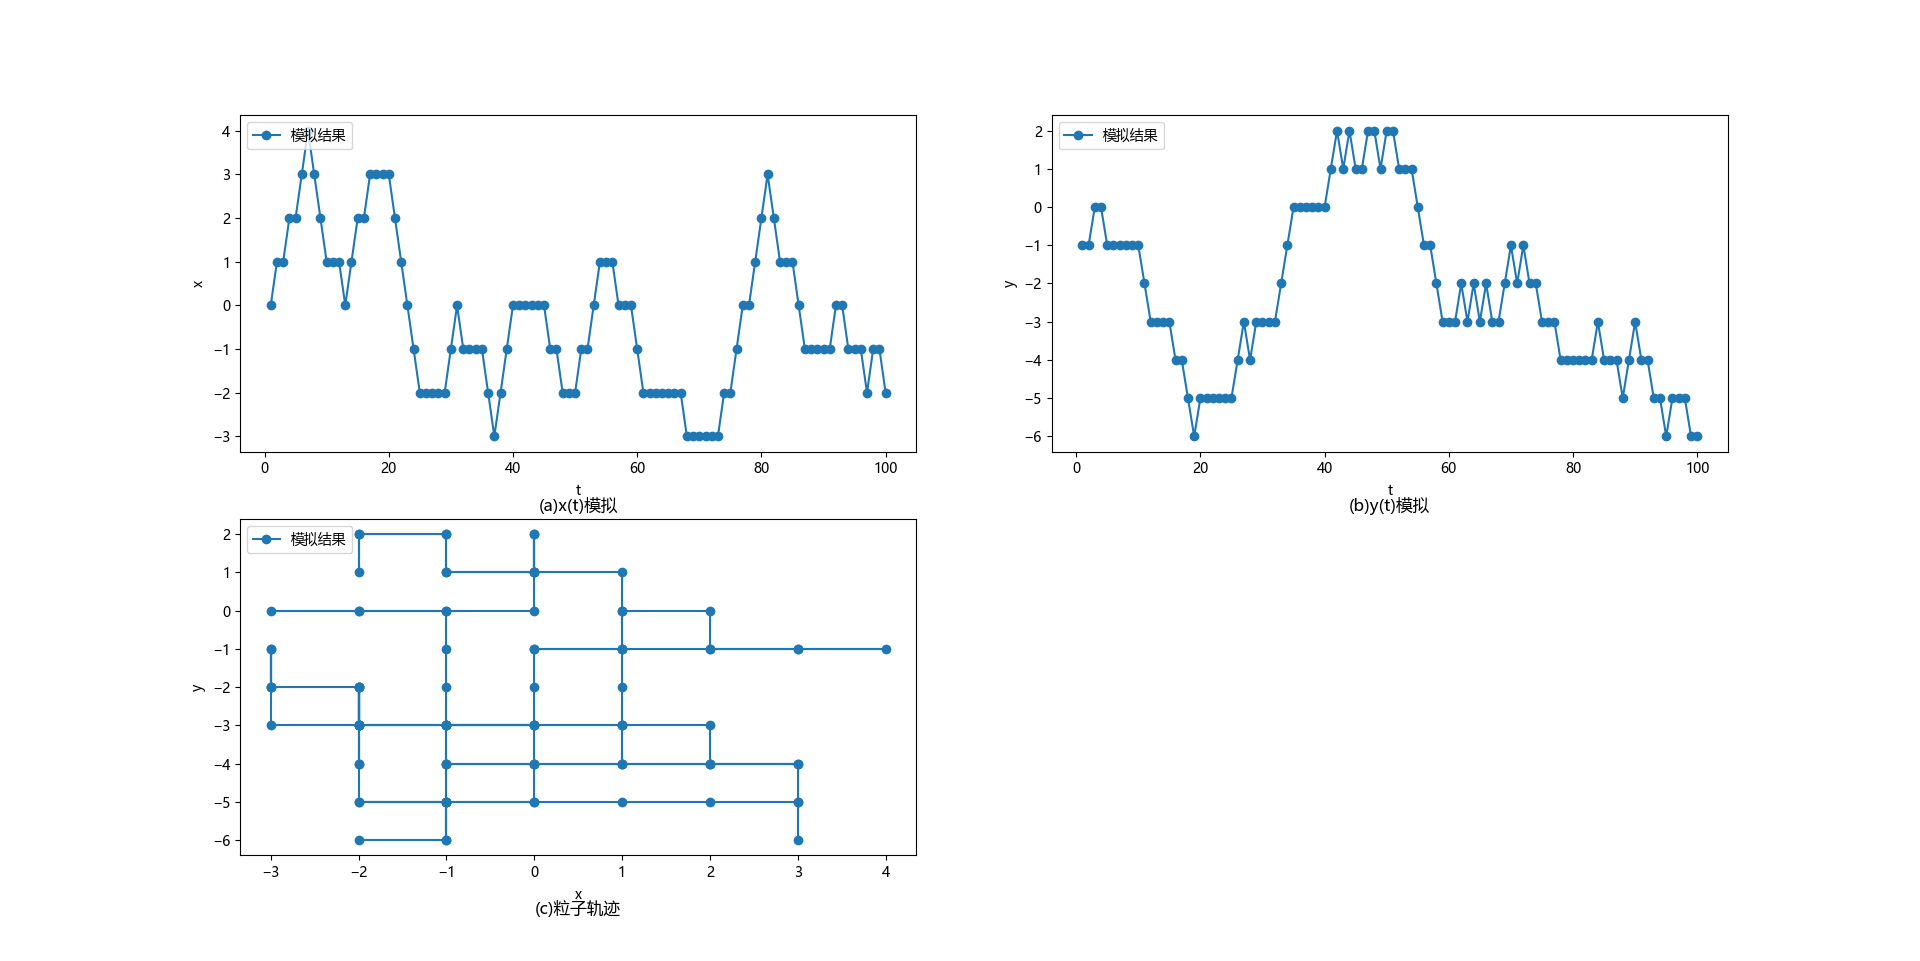
\includegraphics[scale=0.4]{walk}
		\captionsetup{font={small},labelfont=bf}
		\caption{\heiti\zihao{-5}随机游走坐标轨迹}
		\label{fig:1}%label加最后才可以引用正常
	\end{figure}
	这里模拟了$ n=10^5 $个粒子在$ t=1\sim100 $时间段内的随机游走,并且取了在以下不同参数的情况。以下为取了A=1,w=0.1;A=1,w=0.5;A=1,w=1;A=0.5,w=0.5参数下的模拟结果。对应图2,3,4,5。
	
		
	图中分别计算了模拟粒子随机行走的xy方向位移平均值$ \langle \vec{x_{(t)}}\rangle,\langle \vec{y_{(t)}}\rangle $,粒子位移的平方的平均值$ \langle r^2(t)\rangle $,与粒子的位移方差$ Var_r(t) $。由图可见Monte Carlo模拟结果与期望值曲线符合的较好。
	
	
	可见$ \langle \vec{x_{(t)}}\rangle $在x>0部分呈正弦函数状周期性振荡,$ \langle \vec{y_{(t)}}\rangle $则始终保持为0,与无外场p=1 情况下的随机游走相符合。$ \langle \vec{r_{(t)}}^2\rangle $则呈振荡上升的趋势。而$ Var_r(t) $则振动项较小,近似于线性增长的趋势。随着w的增大,相应各项的振荡频率增大,而振荡的幅度也会变小,分析是由于电场变化速率较快,粒子受到同一个方向的力运动的时间变短,导致了在运动更短距离后随即转向,于是振幅减小。相应于振幅减小,$ \langle \vec{r_{(t)}}^2\rangle $上升的速率与振荡也明显减小。
	
	
	而A的改变只影响振荡的振幅,同时A增大会导致$ \langle \vec{r_{(t)}}^2\rangle $与$ Var_r(t) $的上升减缓,振荡增强,这是由于较大的外电场的存在会使粒子更多的向同一方向运动,导致反方向运动的粒子贡献的到原点距离的平方减小,同时粒子整体的通向运动也会导致分布的宽变窄。
		\begin{figure}[!h]
		
		\centering
		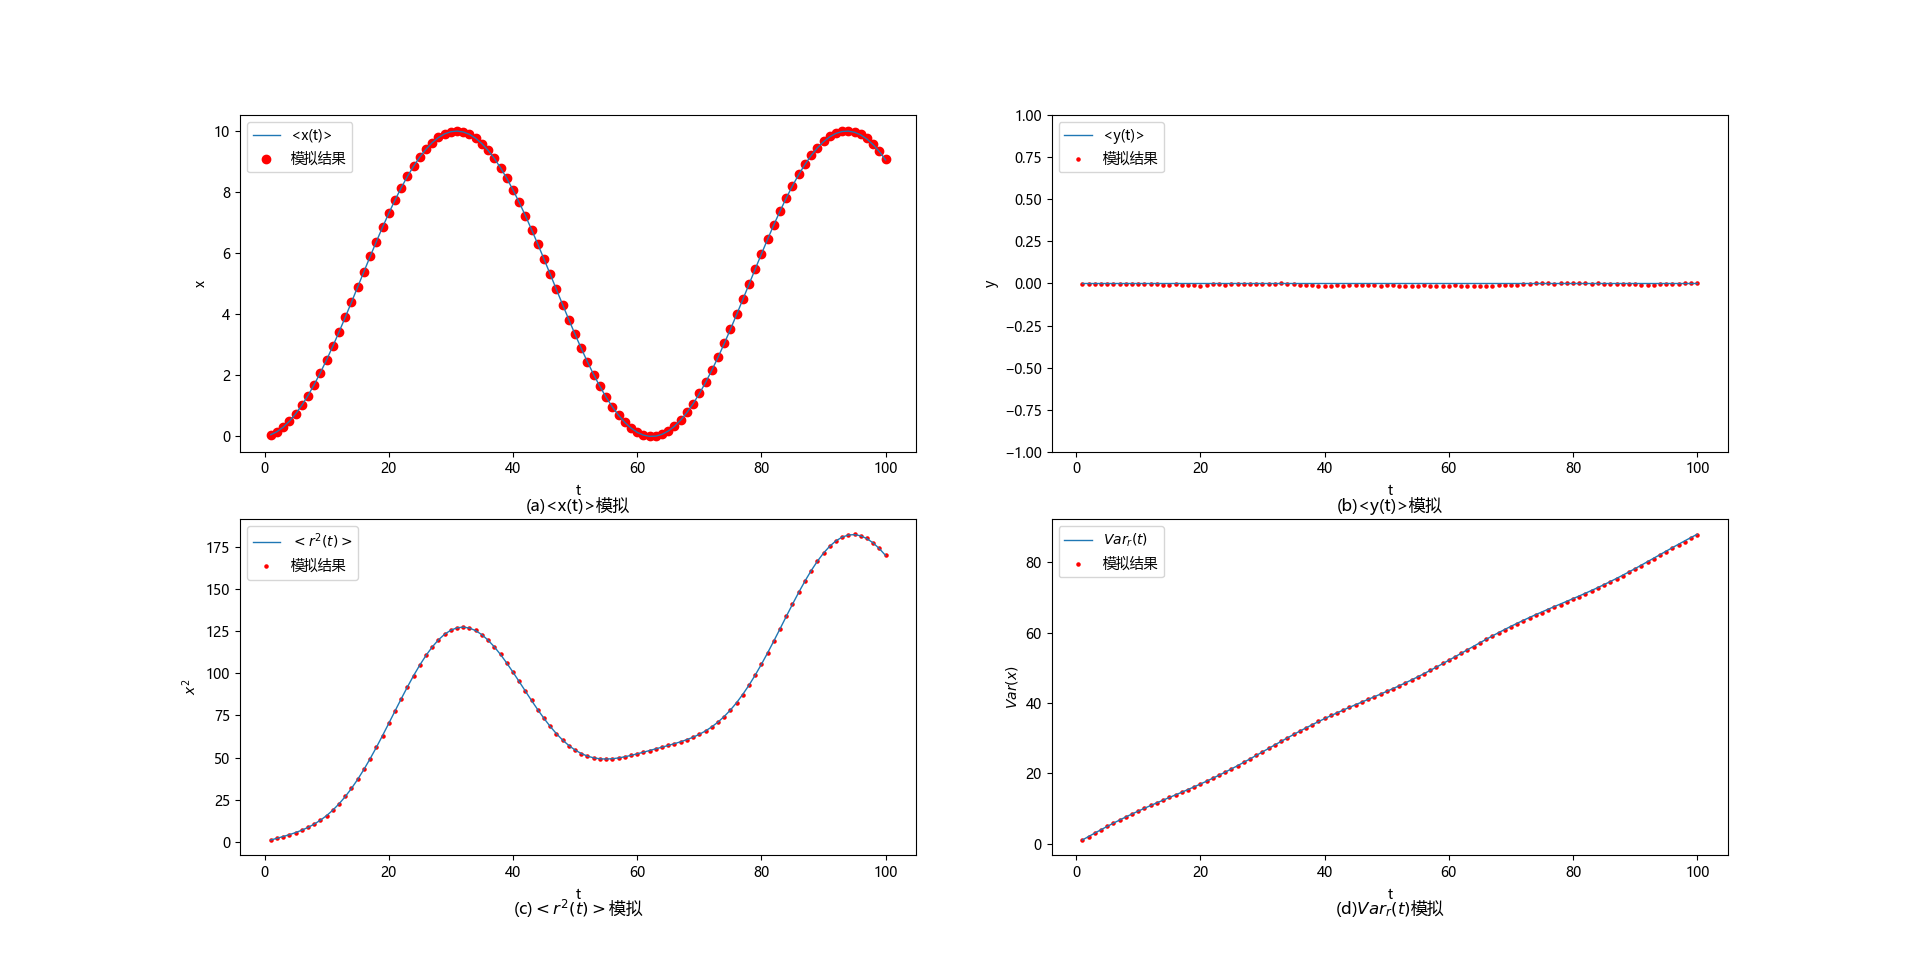
\includegraphics[scale=0.4]{A1w0.1}
		\captionsetup{font={small},labelfont=bf}
		\caption{\heiti\zihao{-5}A=1,w=0.1}
		
	\end{figure}
		\begin{figure}[!h]
	
	\centering
	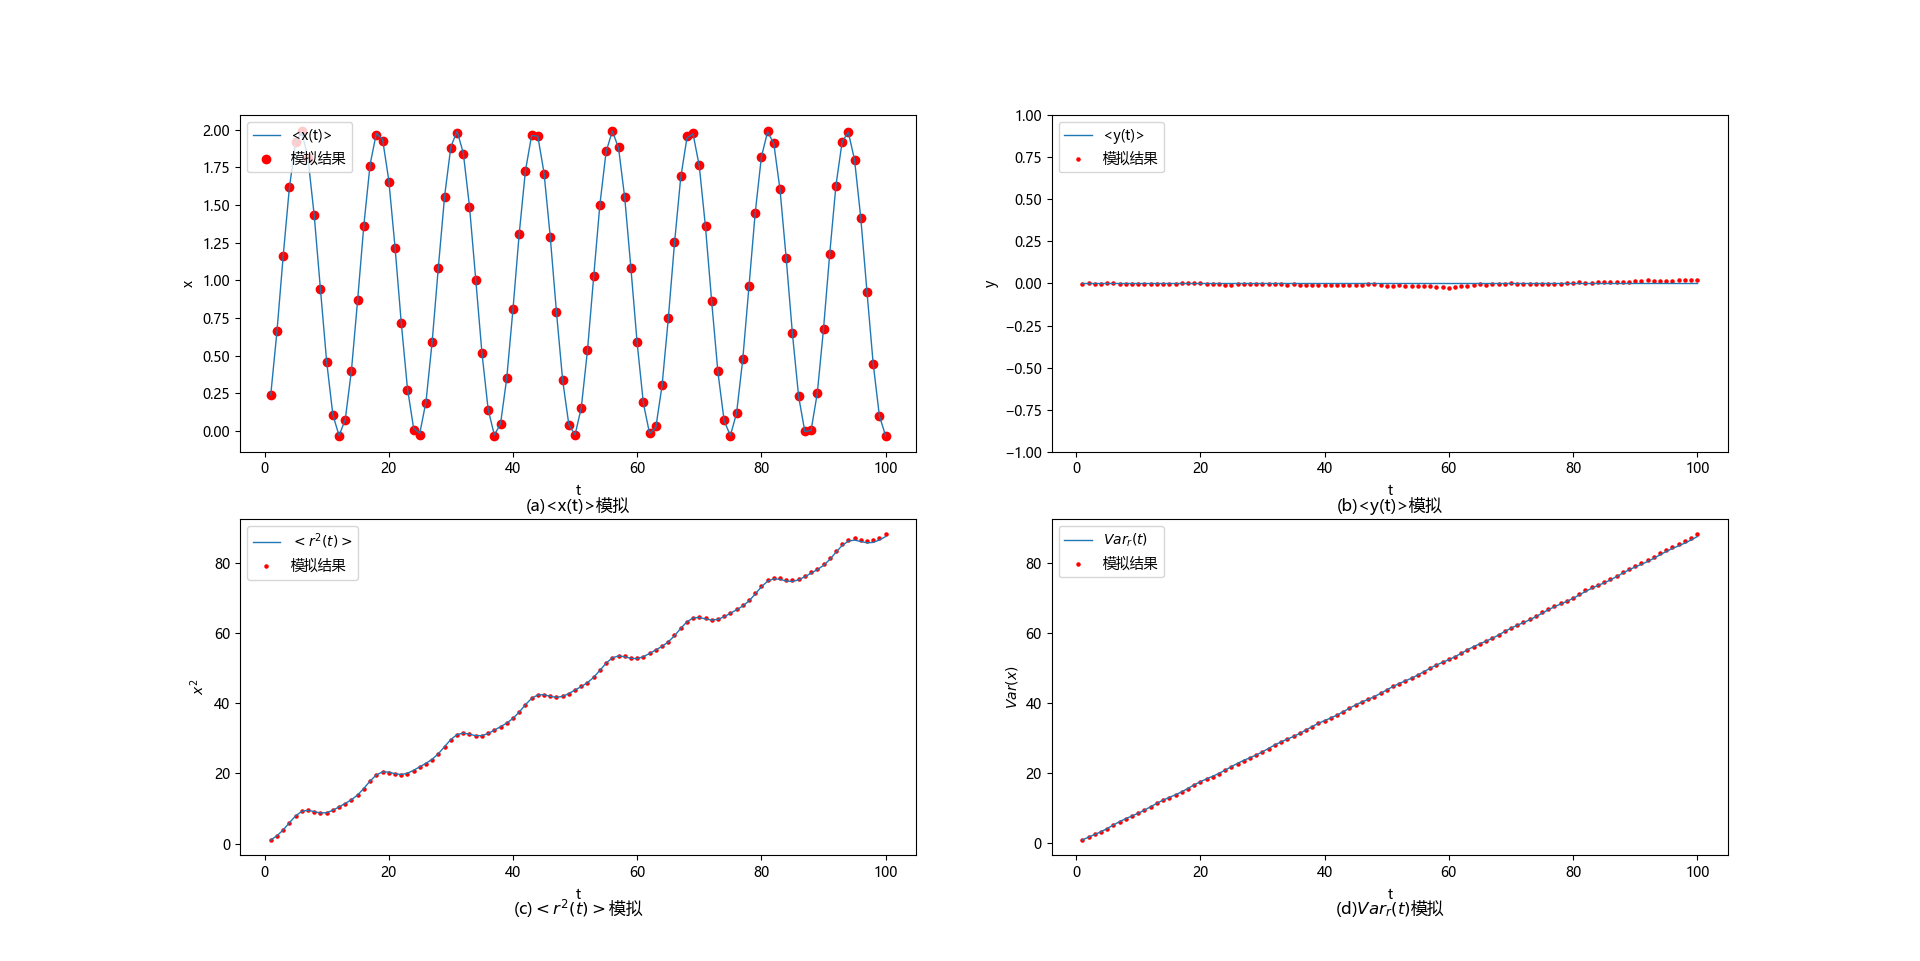
\includegraphics[scale=0.4]{A1w0.5}
	\captionsetup{font={small},labelfont=bf}
	\caption{\heiti\zihao{-5}A=1,w=0.5}
	
\end{figure}
		\begin{figure}[!h]
	
	\centering
	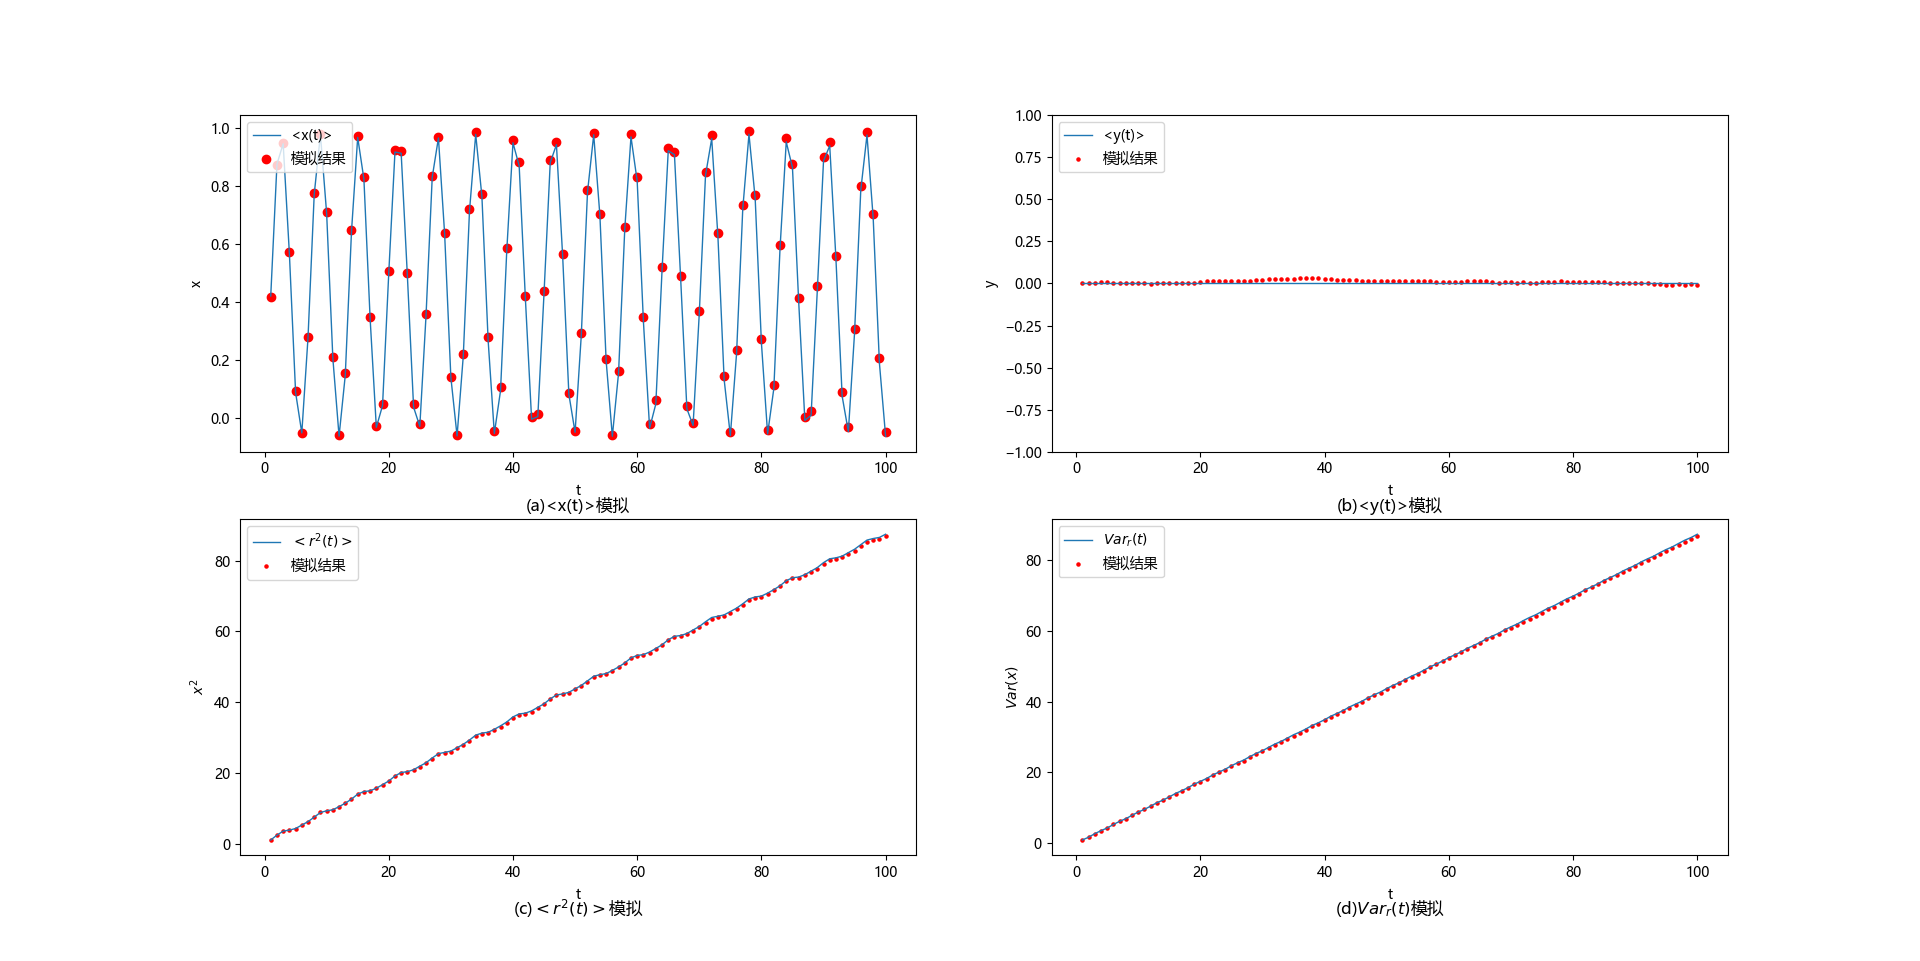
\includegraphics[scale=0.4]{A1w1}
	\captionsetup{font={small},labelfont=bf}
	\caption{\heiti\zihao{-5}A=1,w=1}
	
\end{figure}
\begin{figure}[!h]

\centering
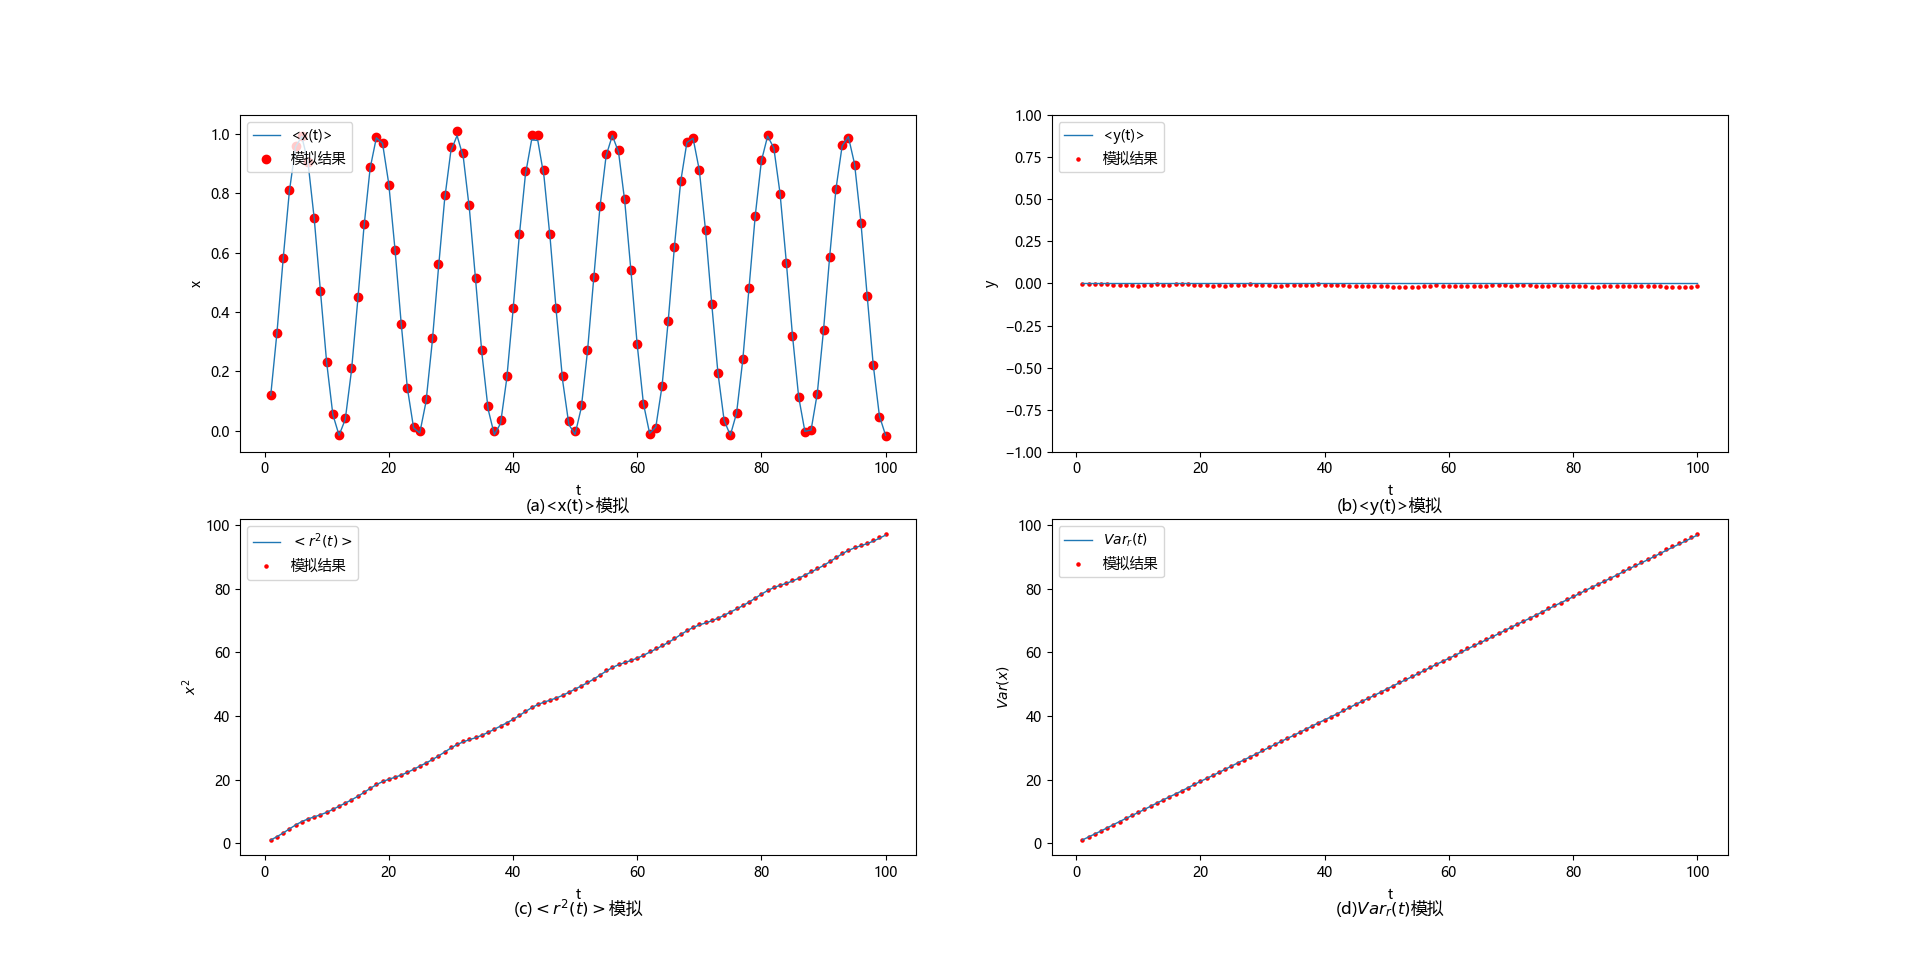
\includegraphics[scale=0.4]{A0.5w0.5}
\captionsetup{font={small},labelfont=bf}
\caption{\heiti\zihao{-5}A=0.5,w=0.5}

\end{figure}


~\\
\newpage
之后统计了该n=$ 10^5 $,t=100,A=1,w=0.5下的模拟结果中粒子在空间的分布如图6
\begin{figure}[!h]
	
	\centering
	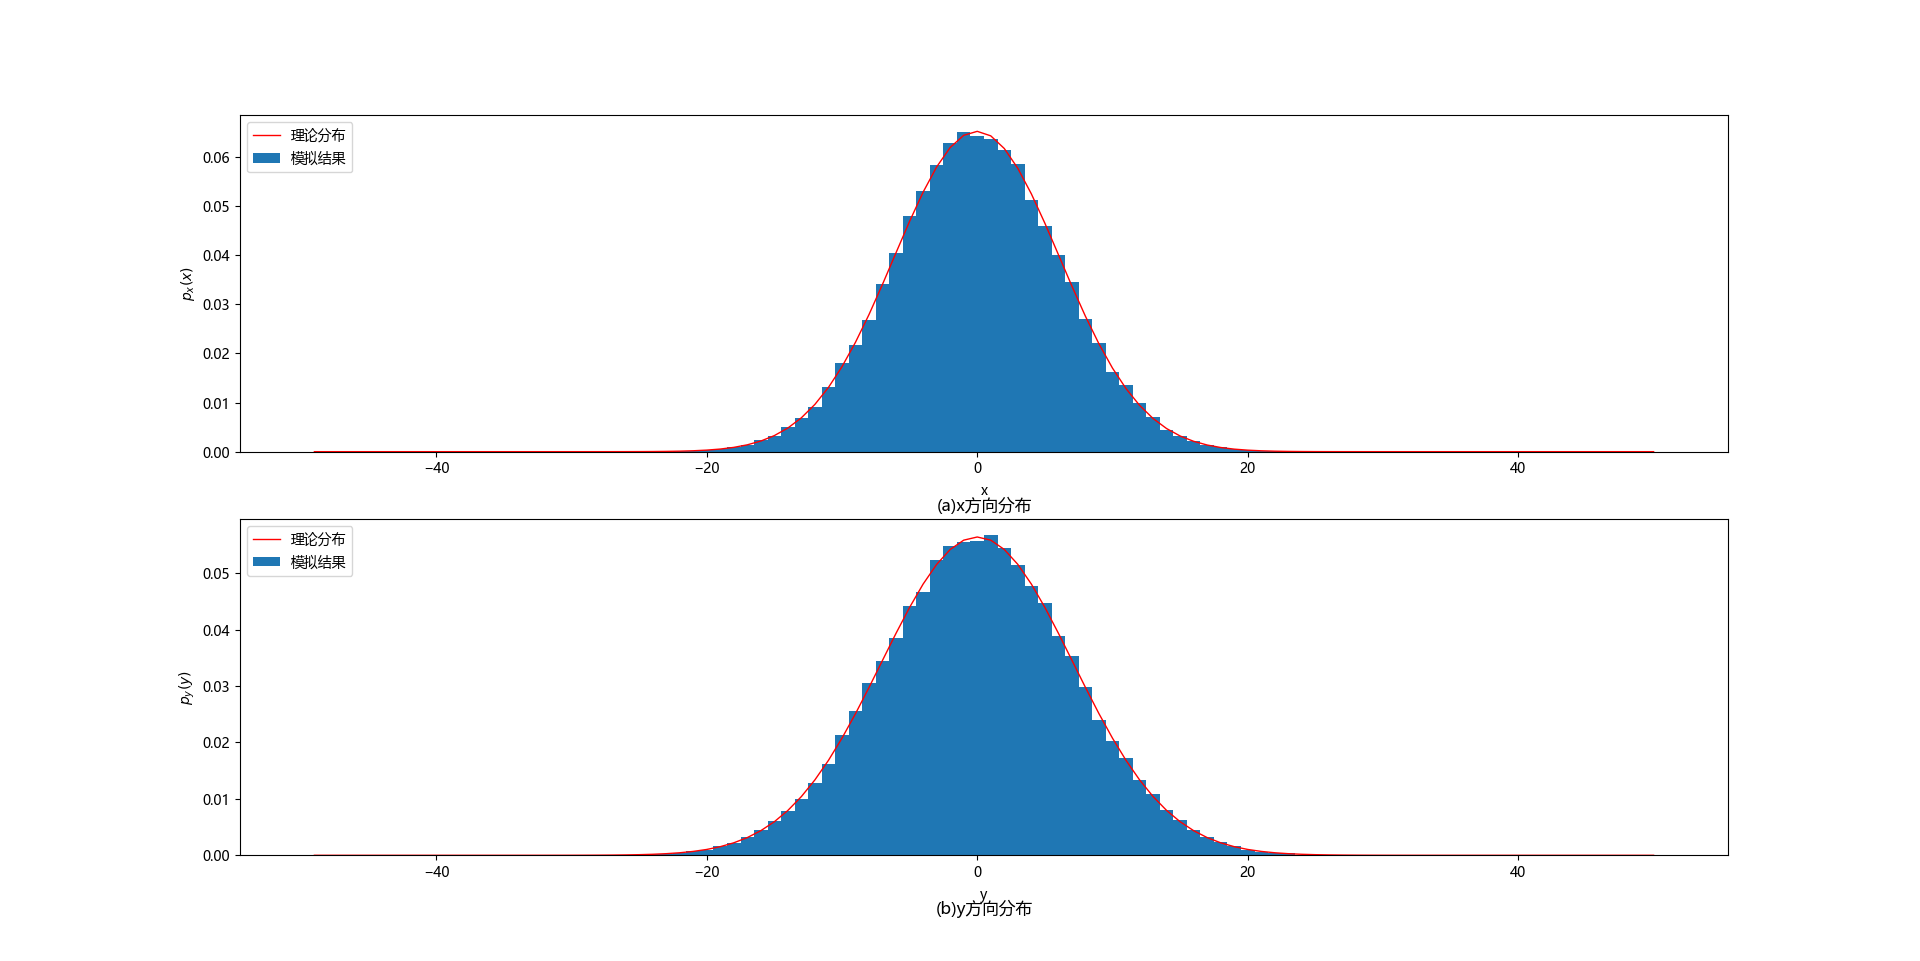
\includegraphics[scale=0.4]{distribution}
	\captionsetup{font={small},labelfont=bf}
	\caption{\heiti\zihao{-5}粒子分布统计}
	
\end{figure}

~\\
根据粒子随机游走的高斯分布结果
\begin{equation}
	p_x(x,t)=\frac{1}{2\pi\sigma_x^2}e^{-(x-\langle x\rangle)^2/2\sigma_x^2}
\end{equation}
\begin{equation}
	p_y(y,t)=\frac{1}{2\pi\sigma_y^2}e^{-(y-\langle y\rangle)^2/2\sigma_y^2}
\end{equation}
其中由上计算式(\ref{eq:4})(\ref{eq:5})(\ref{eq:6})可得
\begin{equation}
	\begin{cases}
		\sigma_x^2=t(1/2-\frac{A^2}{8})+\frac{A^2\sin(wt)\cos(t+1)w}{8\sin(w)}\\
		\sigma_y^2=1/2
	\end{cases}
\end{equation}
\begin{equation}
	\begin{cases}
		\langle x\rangle=\frac{A\sin(\frac{wt}{2})\sin(\frac{t+1}{2}w)}{2\sin(w/2)}\\
		\langle y\rangle=0
	\end{cases}
\end{equation}
可见分布结果符合高斯分布。
\subsection{速度自相关函数模拟}
这里取了初始条件$ v_{x0}=1,v_{y0}=1 $,在A=1,w=0.5下模拟得到的结果如下图7所示,趋势为先指数下降之后,在0附近振荡。
\begin{figure}[!h]
	
	\centering
	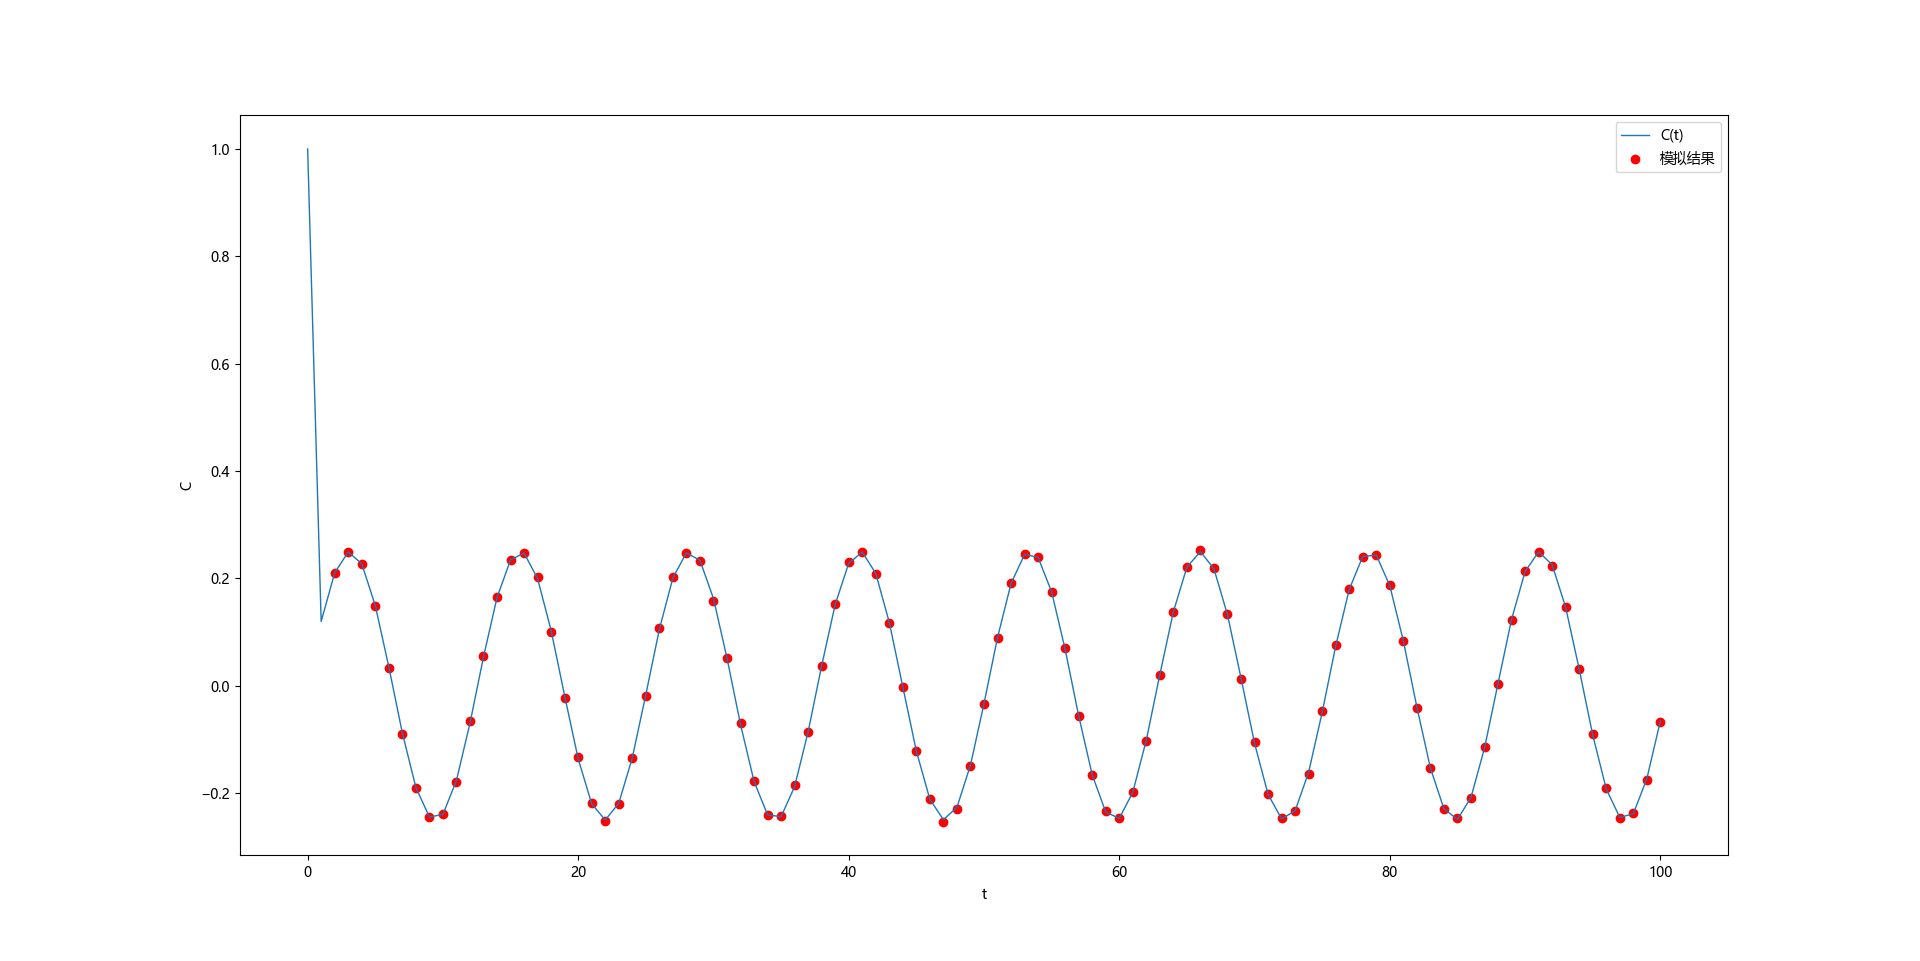
\includegraphics[scale=0.4]{C}
	\captionsetup{font={small},labelfont=bf}
	\caption{\heiti\zihao{-5}速度自相关函数曲线模拟}
	
\end{figure}


这里由于$ \tau=m/\alpha=10^{-7} $为无穷小量,对于式(11)的计算结果可得指数项衰减的很快,将指数项和$ \tau $的二次项省略后即可得到近似的式
\begin{equation}
	C(t)=\frac{1}{2}\langle v_x(0)\rangle\frac{Eq}{m}\tau\sin(wt)
\end{equation}
\begin{figure}[!h]
	
	\centering
	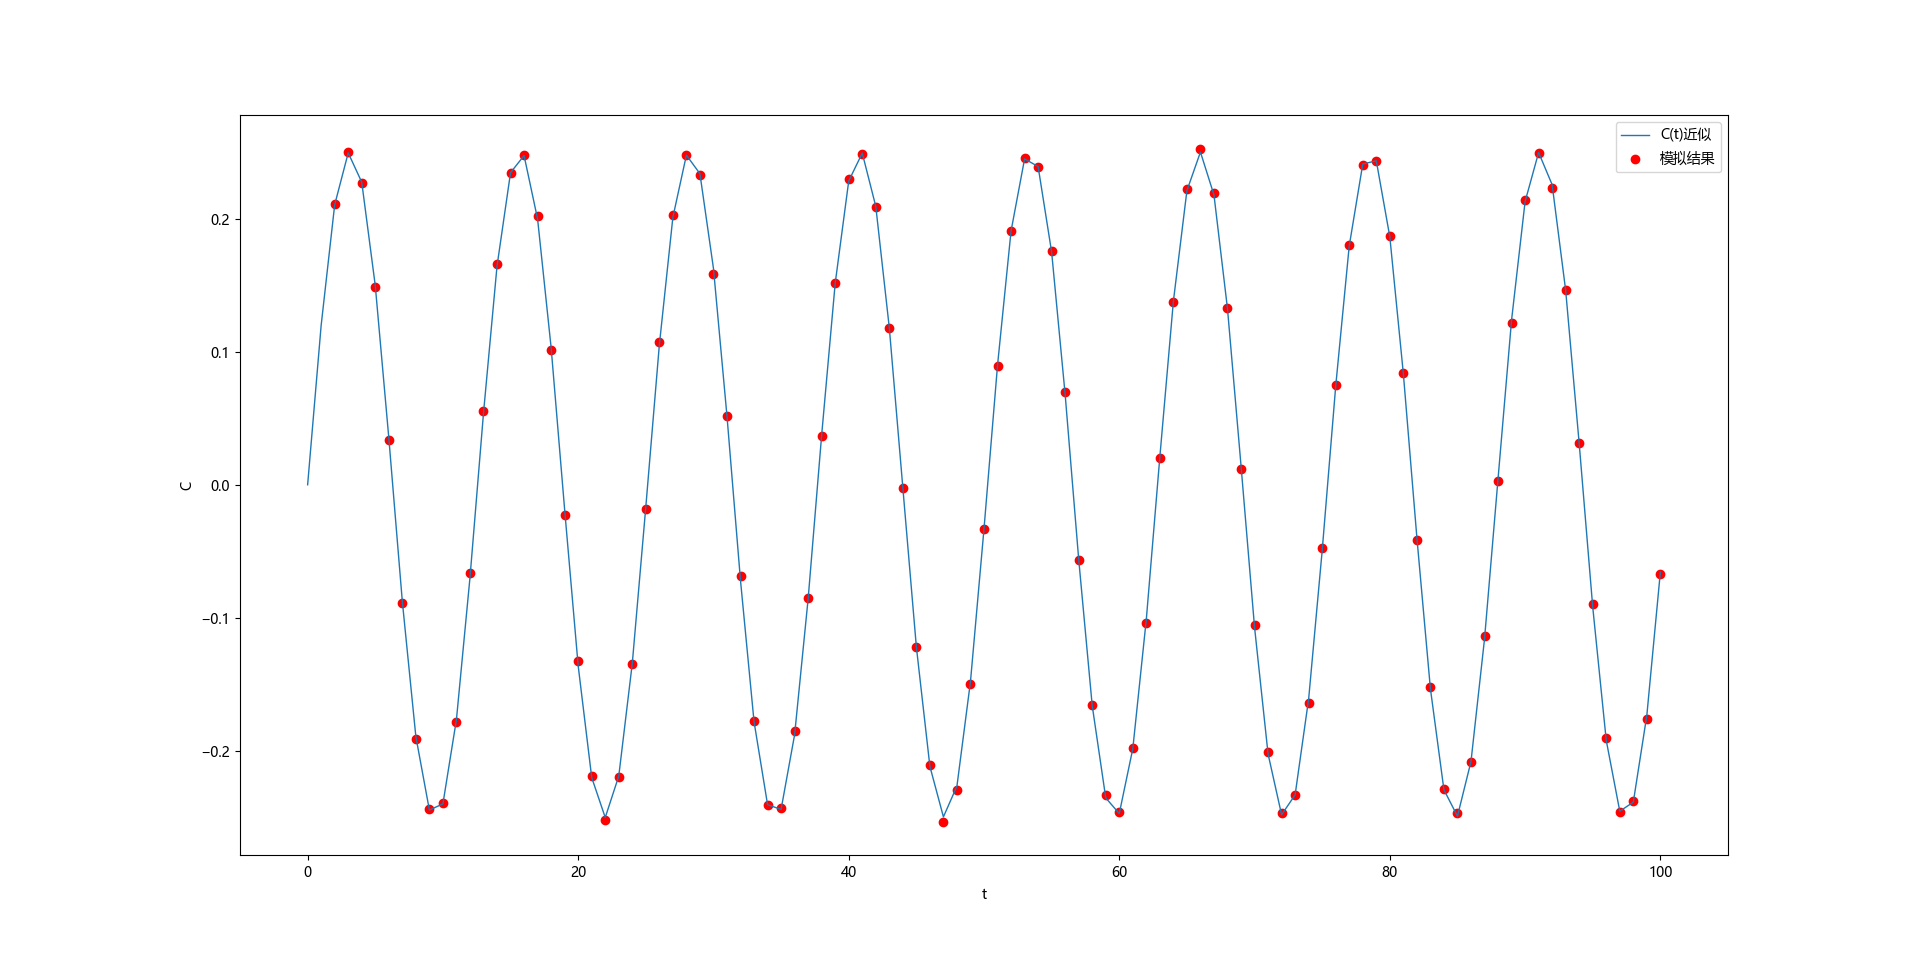
\includegraphics[scale=0.4]{C_approx}
	\captionsetup{font={small},labelfont=bf}
	\caption{\heiti\zihao{-5}速度自相关函数曲线模拟与近似理论结果对比}
	
\end{figure}
可得该近似曲线也与模拟结果和标准理论曲线较为相符。如图8


接下来我们分析了初始时刻粒子速度随机分布的情况,即按照Boltzmann分布
\begin{equation}
	g(v_{x_0},v_{y_0})=\frac{1}{2\pi\sigma}\exp(-\frac{v_{x_0}^2+v_{y_0}^2}{2\sigma^2})
\end{equation}
根据初速度分布有$ \langle v_{0}\rangle=0,\langle v_0^2\rangle=2\sigma^2 $得到速度自相关函数为
\begin{equation}
	C(t)=\sigma^2\exp(-\frac{t}{\tau})
\end{equation}
模拟结果如图\ref{fig:9}所示,呈指数下降趋势,基本与外电场无关。
\begin{figure}[!h]
	
	\centering
	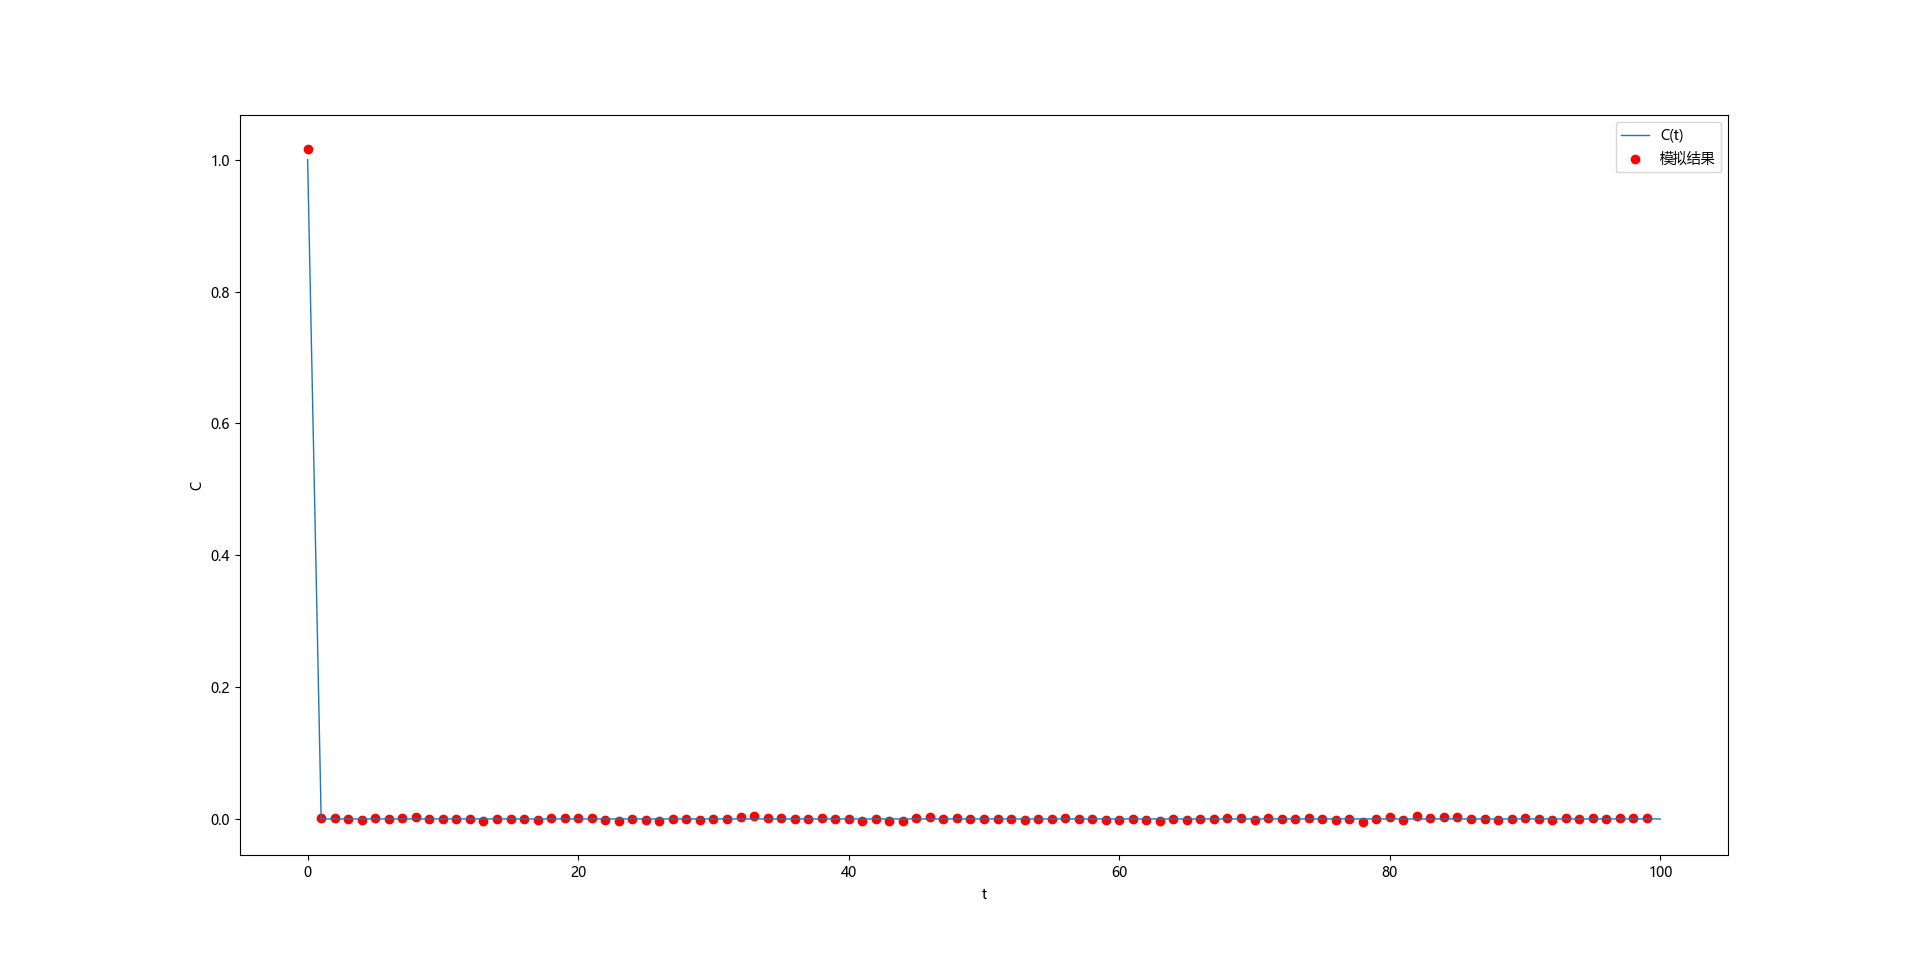
\includegraphics[scale=0.4]{C_rand}
	\captionsetup{font={small},labelfont=bf}
	\caption{\heiti\zihao{-5}速度自相关函数曲线模拟与近似理论结果对比}
	\label{fig:9}
\end{figure}
	\section{结论}
	本次实验利用Monte Carlo方法模拟粒子在偏压下随机行走,分析了粒子在正弦外电场偏压下随机游走的同时产生的一定周期性振荡,并且分析了电场大小与频率对粒子运动均值、方差的一些影响。
	
	
	同时模拟结果发现在偏压下随机游走的粒子空间分布情况仍然符合Gauss分布的形式,仅仅是外场对粒子的位移均值、方差有一定的影响,但与分布形式无关。
	
	
	最后进行了速度自相关函数的模拟。首先进行了设定所有粒子具有初速度$ v_{x_0}=v_{y_0}=1 $的情况,模拟的结果和所对比的理论曲线均为精确结果,但是发现进行了$ \tau $为小量的近似后发现仍然与精确结果和模拟结果相近,几乎只存在正弦振荡的项。实际上我们可以发现,有外电场的作用下,由于粒子很轻,即$ \tau\sim10^{-7} $,会导致粒子在电场下迅速加速使所受的粘滞阻力与电场力保持平衡,于是粒子的速度以及自相关函数基本完全受到外场变化规律的控制。接下来按照玻尔兹曼分布模拟了粒子的初始速度,发现结果与粒子所在的外场基本无关,呈指数下降趋势。说明粒子初始的速度分布状况会很大程度上影响粒子速度自相关函数的性质。
\end{document}